\documentclass[11pt]{article}

\usepackage[english]{babel}
\usepackage[utf8]{inputenc}
\usepackage{amsmath}
\usepackage{amssymb}
\usepackage{graphicx}
\usepackage[colorinlistoftodos]{todonotes}
\usepackage{listings,multicol}
\usepackage{textcomp}
\usepackage{hyperref}

\setlength{\oddsidemargin}{0.5cm} \setlength{\evensidemargin}{0cm}
\setlength{\textwidth}{16cm} \setlength{\textheight}{23cm}
\setlength{\topmargin}{-0.5cm}
\textheight 21.5cm


\usepackage[numbered,framed]{matlab-prettifier}
\lstMakeShortInline"
\lstset{
  style              = Matlab-editor,
  %basicstyle         = \mlttfamily,
  escapechar         = ",
  mlshowsectionrules = true,
}

\begin{document}

\title{T1 NUMERICO UBB 220138}

{\begin{minipage}{2cm}
\hspace*{1cm}
\includegraphics[width=0.6\textwidth]{escubo-ubb.eps}
\end{minipage}
\begin{minipage}{12cm}
\small
{\bf \rm 
{
\begin{center}
{\footnotesize UNIVERSIDAD DEL B\'IO-B\'IO} \\
{\scriptsize FACULTAD DE CIENCIAS}  \\
{\scriptsize DEPARTAMENTO DE MATEM\'ATICA}  \\
{\scriptsize Profesor:  Franco Milanese}\\
{\scriptsize Ayudantes: Isabella Ferrari, Mario Valdés}\\
{\scriptsize Segundo Semestre de 2016}
\end{center}
}}
\end{minipage}}
{\begin{minipage}{2cm}
\hspace*{-0.5cm}\vspace*{-0.05cm}
\includegraphics[width=0.7\textwidth]{escudo-dmat.eps}
\end{minipage}}

\hspace*{-1,5cm}\rotatebox[origin=c]{90}{\begin{picture}(0,0)
\put(0,7){\makebox(9,-13)[l]{\hspace*{-6.5in} \bf \it Departamento de Matem\'atica - Universidad del B\'io-B\'io - 2016}}
\end{picture}}

\vspace*{0.5cm} \centerline {\bf\underline{Test 1 versión 1, Taller de Ciencias }}
\centerline{\textrm{Semana 26-30 de Diciembre}}  \vspace{0.2cm}


\begin{center}
 \begin{tabular}{p{0.7\textwidth}p{0.3\textwidth}}
	\textbf{Nombre:}   &\textbf{Carrera:}\\ \\
	\textbf{Ayudante:} & \textbf{ RUT:}
 \end{tabular}
 \\
 \vspace{0.2cm}
 \begin{tabular}{||p{2cm}|p{2.1cm}|p{2.1cm}||p{2cm}||}
 \hline
 Pregunta 1 &  Pregunta 2a &    Pregunta 2b & Total\\
 \hline
 \vspace{1.5cm} & & &    \\
 \hline
 \end{tabular}
 \end{center}
 Enviar archivos solicitados en el formato solicitado a \textbf{veranonumerico@gmail.com}.

\begin{enumerate}
\item (30 pt) Descargue el archivo ubicado en 
\begin{center}
\url{http://www.udec.cl/~fmilanese/mop.xlsx}
\end{center}
este contiene el detalle de los contratos de obras, estudios y asesorías pagados por el Ministerio de Obras Públicas de Chile durante abril de 2016.
\begin{enumerate}
	\item (5 pt) En un rutero llamado \texttt{mop.m} cargue a Matlab el archivo descargado usando el comando \texttt{xlsread()}.
    \item (15 pt) En el mismo rutero ingrese las instrucciones para generar las gr\'aficas de los montos cancelados por el \textbf{MOP} versus el día en el que se realizaron con asteriscos azules. Observará que la fecha está contada en una enumeración de días, utilice el comando \texttt{datetick('x')} para visualizar la fecha en la gráfica. 
    \item (5 pt) Grabe la figura generada como \texttt{mop.jpg} .
    \item (5 pt) Responda a continuaci\'on la siguiente pregunta ¿Qu\'e empresa y regi\'on se adjudicó el mayor monto por concepto de contrato de obra, estudio o asesoría en el periodo descargado?.

\fbox{ \begin{minipage}{0.8\textwidth}  

\hfill\vspace{2cm} 
\end{minipage} } 
    
\end{enumerate}
Adjunte el programa \texttt{mop.m} y la imagen \texttt{mop.jpg} al correo.

\textbf{Desarrollo:} El programa \texttt{mop.m} debe contener las instrucciones
\begin{lstlisting}
[NUM,TXT,RAW]=xlsread('mop.xlsx');
plot(NUM(:,4),NUM(:,end),'*b');
datetick('x');
[monto,index]=max(NUM(:,end))
RAW(index+1,1)
RAW(index+1,end-1)
\end{lstlisting}
con lo cual se genera la gr\'afica
\begin{center}
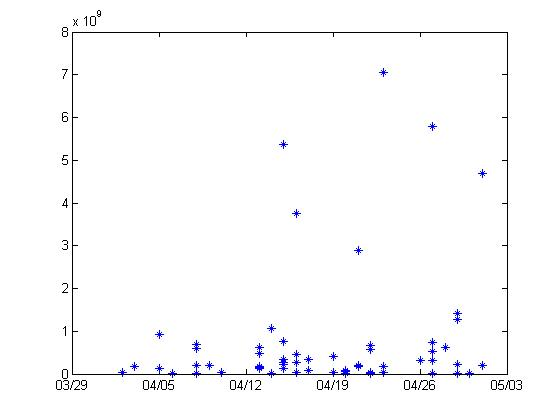
\includegraphics[width=0.75\textwidth]{./mop.jpg}
\end{center}
y de donde se deduce que
\begin{lstlisting}
ans = 

    'Antofagasta'


ans = 

    'INGENIERIA Y CONSTRUCCION TRIOVIAL LTDA.'

\end{lstlisting}

\newpage
\item (20 pt) Resuelva uno, y sólo uno, de los siguientes problemas.
\begin{enumerate}
\item
En un rutero de Matlab llamado \texttt{p2.m} grafique las funciones
\begin{multicols}{2}
	\begin{enumerate}
    	\item $f(x)=sin(x^2)$,
        \item $g(x)=f(x)/(x^2+1)$,
        \item $h(x)=f(2x+1)$,
        \item $i(x)=cos(f(x))$.
    \end{enumerate}
\end{multicols}
La gr\'afica de las funciones debe realizarse en una misma figura en cuatro gr\'aficos distintos y sobre el intervalo $[-\pi,\pi]$. Grabe la figura generada como \texttt{p2.jpg}.

Adjunte el programa \texttt{p2.m} y la imagen \texttt{p2.jpg} al correo.

\textbf{Desarrollo:} El programa \texttt{p2.m} debe contener instrucciones como
\begin{lstlisting}
clear all; close all; clc;
f= @(x) sin(x.^2);
x=-pi:0.01:pi;
subplot(2,2,1);
plot(x,f(x));
subplot(2,2,2);
plot(x,f(x)./(x.^2+1));
subplot(2,2,3);
plot(x,f(2*x+1));
subplot(2,2,4);
plot(x,cos(f(x)));
\end{lstlisting}
las cuales permitan construir la gr\'afica
\begin{center}
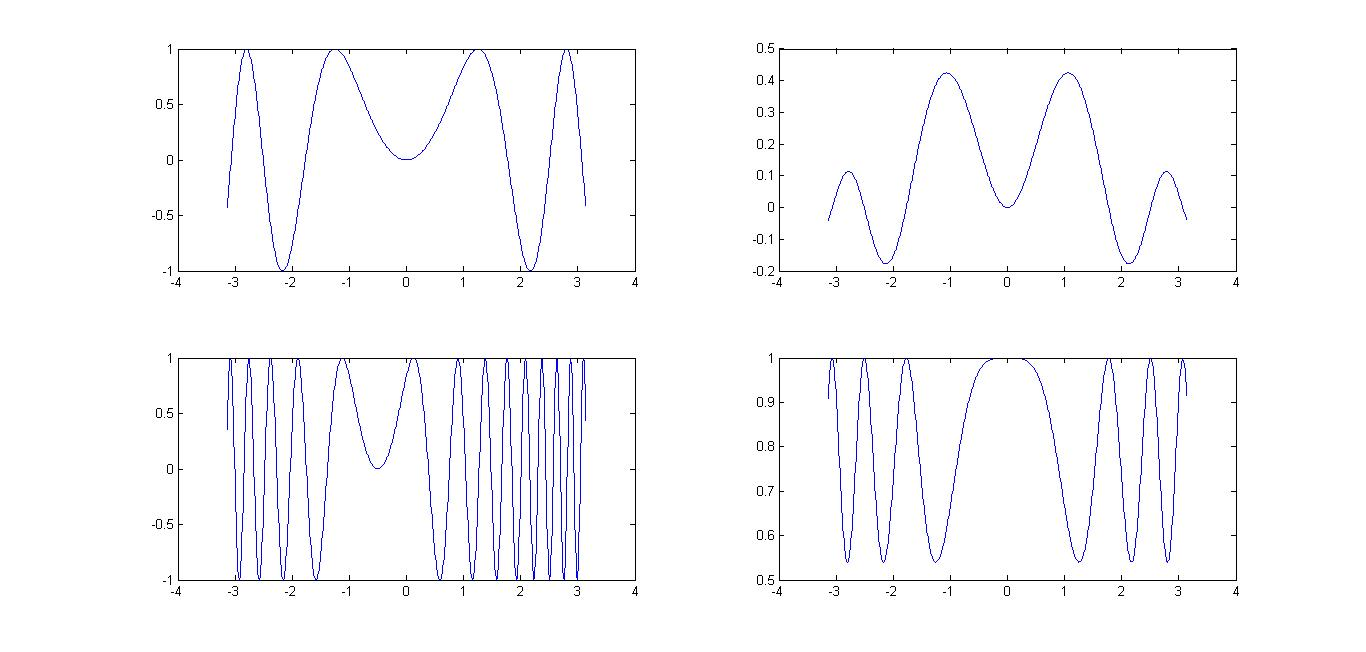
\includegraphics[width=0.75\textwidth]{./p2.jpg}
\end{center}

\vspace{1cm}
\item Cree una funci\'on de Matlab llamada \texttt{creador} la cual al ejecutarse de la forma \texttt{creador(n)} retorne una matriz que tenga la siguiente estructura
$$
\begin{bmatrix}
1 & 2 & 3 & 4 & \cdots & n-1 & n\\
n+1 & n+2 & n+3 & n+4 & \cdots & 2n-1 & 2n\\
n	& n-1 & n-2 & n-3 & \cdots & 2 & 1\\
2n	& 2n-1 & 2n-2 & 2n-3 & \cdots & n+2 & n+1\\
\end{bmatrix}_{4\times n},
$$
donde $n$ es un n\'umero natural. 

Adjunte la funci\'on \texttt{creador.m} al correo.

A continuaci\'on escriba la matriz \texttt{B} generada por la instrucción 
\begin{lstlisting}
A=[creador(5);creador(2),creador(3)];
B=[A;A]'+ones(5,16);
\end{lstlisting}
si existe algún error en esta instrucci\'on justifíquelo.

\vspace{5mm}
\fbox{ \begin{minipage}{0.9\textwidth}  
\hfill\vspace{8cm} 
\end{minipage} } 

\textbf{Desarrollo:} El fichero \texttt{creador.m} debe contener la funci\'on 
\begin{lstlisting}
function A=creador(n)
A=[1:n;n+1:2*n;n:-1:1;2*n:-1:n+1];
end
\end{lstlisting}
con la cual al hacer las instrucciones mencionadas retorna
$$
\left[
\begin{array}{cccccccccccccccccccccccccccccc}
2 & 7 & 6 & 11 & 2 & 4 & 3 & 5 & 2 & 7 & 6 & 11 & 2 & 4 & 3 & 5  \\
3 & 8 & 5 & 10 & 3 & 5 & 2 & 4 & 3 & 8 & 5 & 10 & 3 & 5 & 2 & 4  \\
4 & 9 & 4 & 9 & 2 & 5 & 4 & 7 & 4 & 9 & 4 & 9 & 2 & 5 & 4 & 7  \\
5 & 10 & 3 & 8 & 3 & 6 & 3 & 6 & 5 & 10 & 3 & 8 & 3 & 6 & 3 & 6  \\
6 & 11 & 2 & 7 & 4 & 7 & 2 & 5 & 6 & 11 & 2 & 7 & 4 & 7 & 2 & 5  \\
\end{array}
\right]
$$

\end{enumerate}
\end{enumerate}
\end{document}   
